\documentclass{article}
\usepackage[utf8]{inputenc}

\title{Advanced Programming Labwork 5}
\author{Tom HERBRETEAU }
\date{November 2018}

\usepackage{natbib}
\usepackage{graphicx}
\usepackage{pgfplots}
\pgfplotsset{compat=newest}

\begin{document}

\maketitle
Every performance measures are done on ICT4 with eiffel.jpg, without counting the image saving.
\section{Introduction}
We implement the gaussian blur using cuda. There is two implementation, the first using an array in each thread, and the second with a shared array between every threads in a block using cache memory.
\section{Implementation}
The kernel is launch with 1024 threads per block. For each pixel, it will loop to get the 7x7 pixels around, grayscale it, and make the sum of all 49 px multiply by coef gives by the gaussian matrix filter.
\newline
The difference between the two kernels is the second use shared memory to store the gaussian matrix. The first 49 threads of each blocks will copy it from slow memory to cache memory (faster memory) then we synchronize threads and we can use the cache to compute convolution.
\newline
A way to optimize this process is to grayscale the image before, because it process the grayscale 49 time per pixel instead of 1 (in the grayscale kernel).

\section{Result}
The process time is around 22.1ms for the first kernel, and 22.8 for the second with the shared memory. Actually it's not worth to copy a small array to the cache, because the copy last longer than the time earned by compute with cache array.
\newline
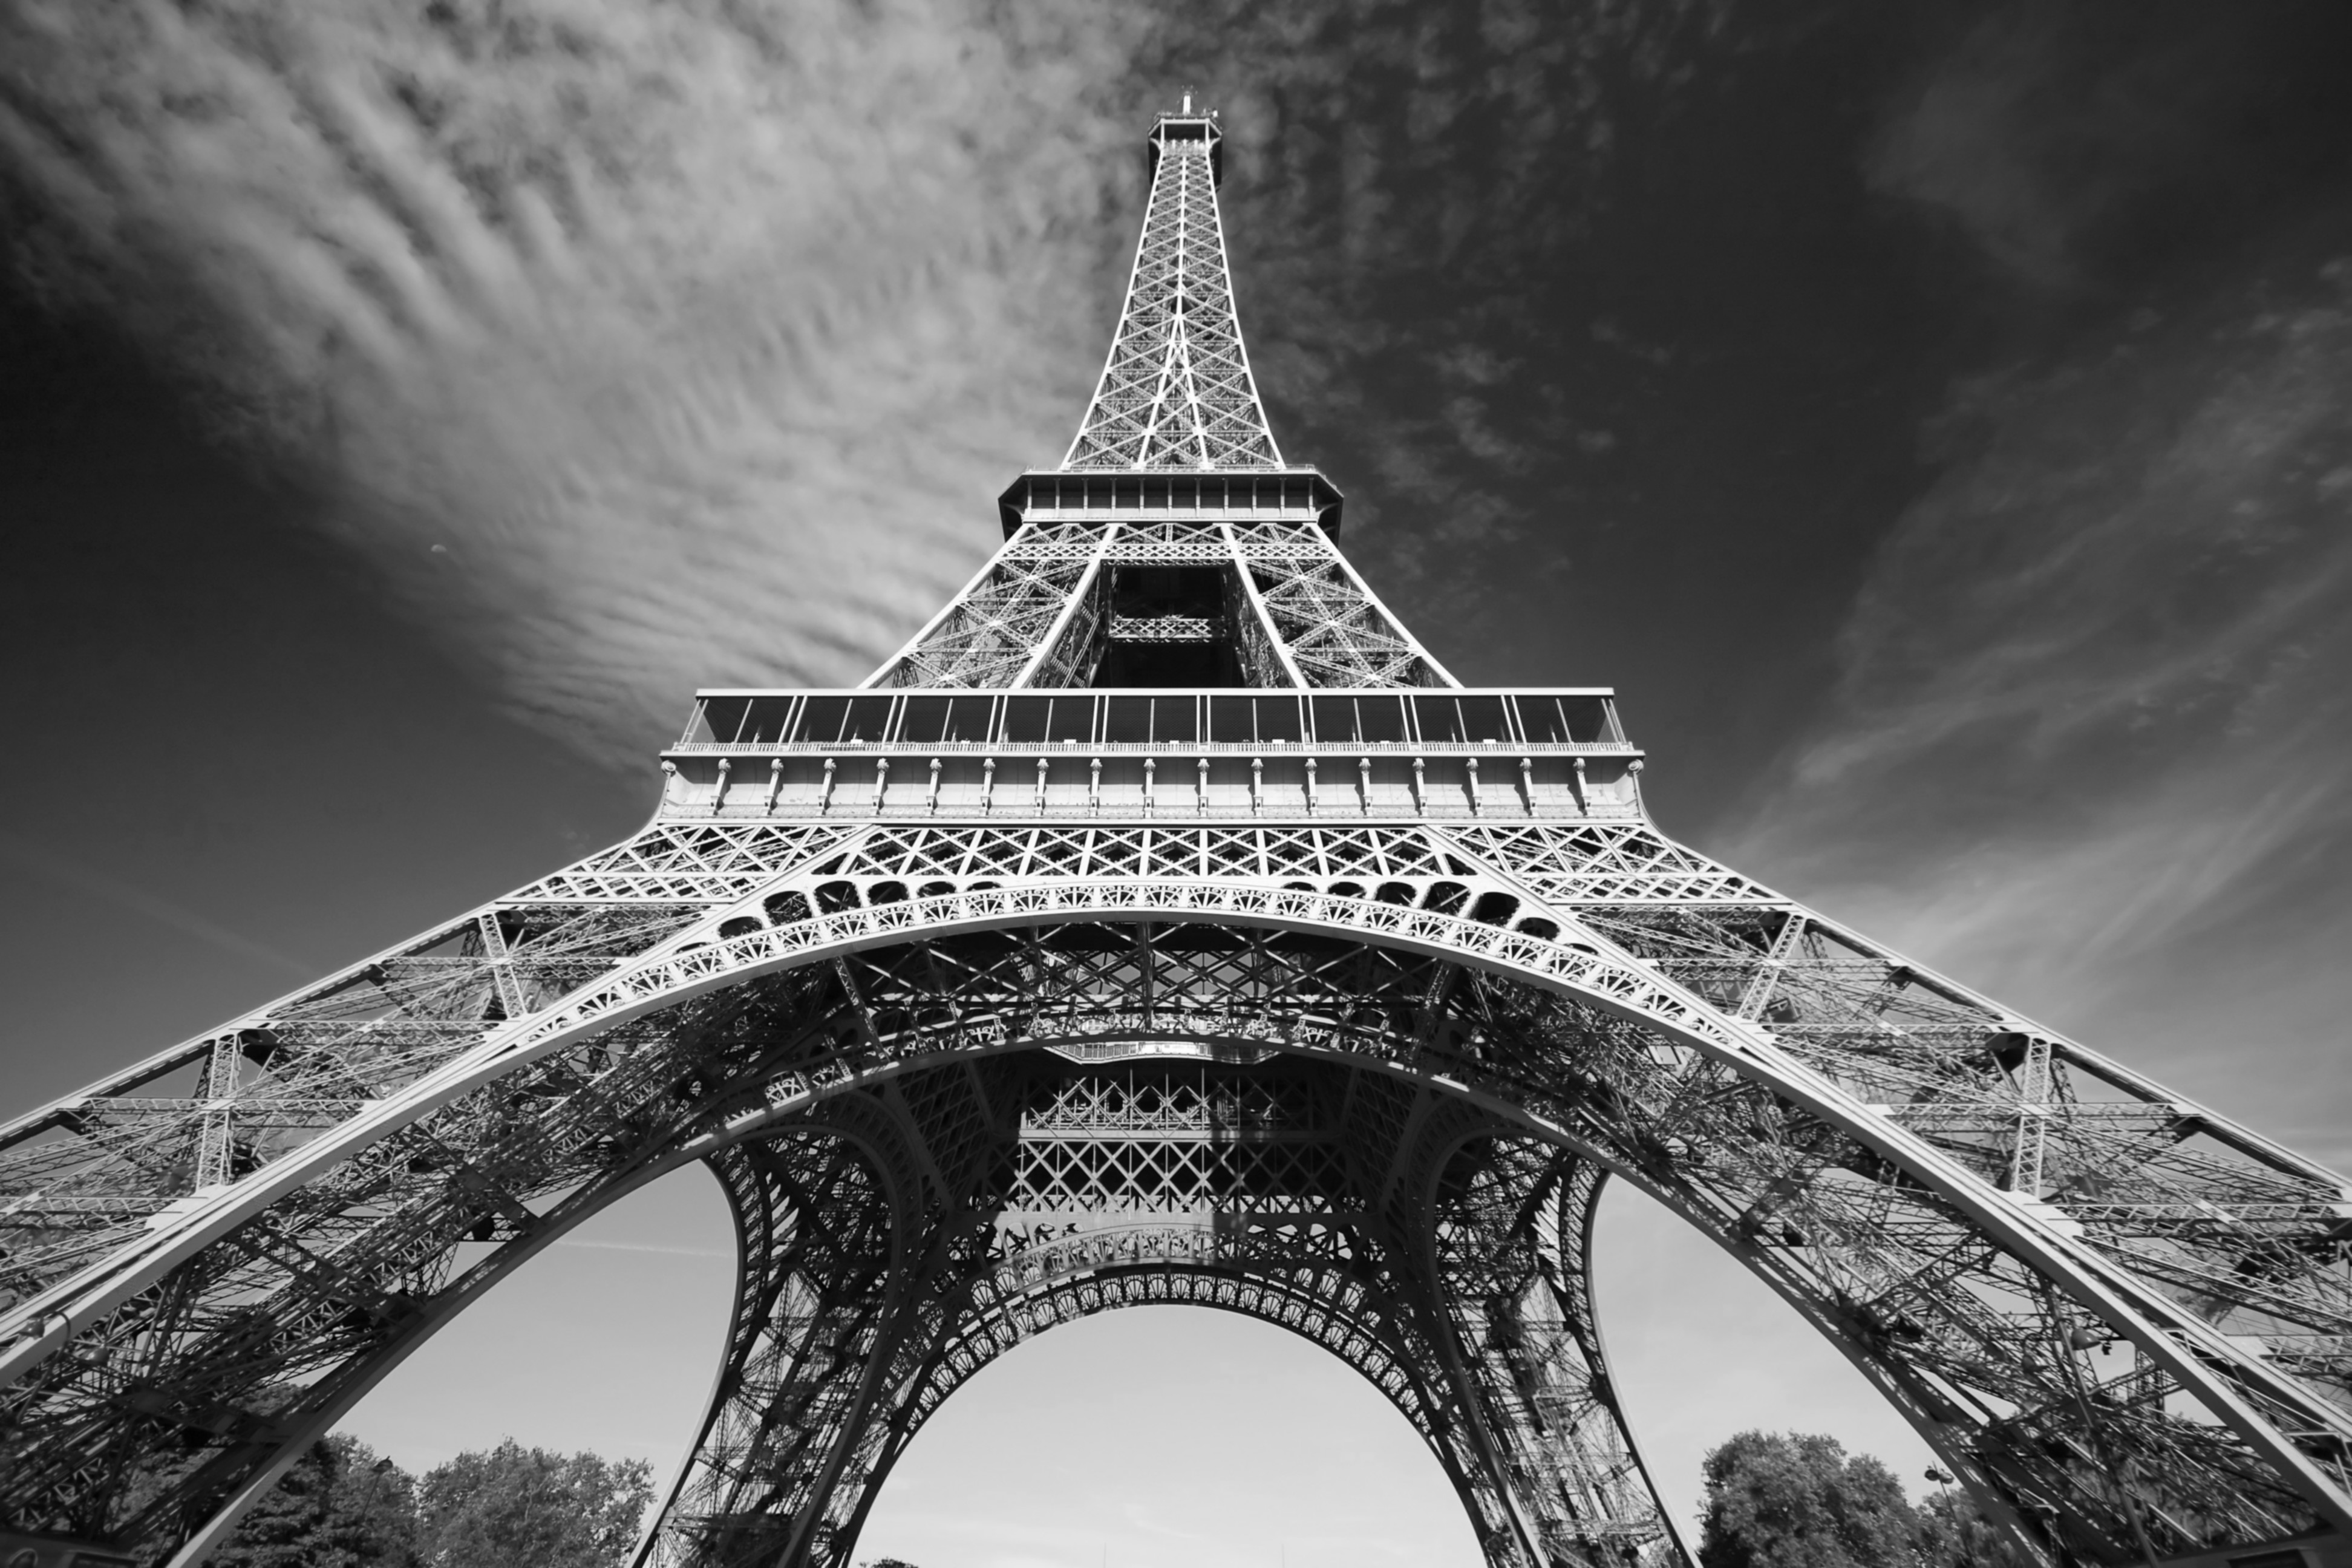
\includegraphics[width=\textwidth]{labwork5-gpu-out.jpg}
\bibliographystyle{plain}
\end{document}
